\documentclass[letterpaper]{article}
\usepackage{notes}
\begin{document}

\section*{Problem Statement}

Consider the dynamic epistemic language
\[
    p \mid \neg \varphi \mid \varphi \land \psi \mid \Know{\varphi} \mid \Typ{\varphi} \mid \Update{P} \varphi
\]
$\KnowNoArgs$ is knowledge.  $\TypNoArgs$ is more interesting --- $\Typ{\varphi}$ says that the current world is `minimal' or `most typical' over worlds satisfying $\varphi$.  (As far as I can tell, this is not quite the same as the $\BestNoArgs$ operator, see Remark 10 in \cite{van2007beliefrevision}).  $\Update{P}$ is some dynamic update given by $\Model \to \Model^\star_P$ (this is a free variable; the problem will be to find the right update).

For the static part of the logic, choose your favorite semantics --- plausibility models, evidence models, etc.  For now, I'll take Johan's approach from \cite{van2011logical}, which I've been using as a desk reference for all this.  Let's assume we have a single-agent plausibility model, with an extra accessibility relation $R$ for knowledge: $\Model = \langle W, R, \leq, V \rangle$.  $\leq$ is uniform over all states; we do not have a different plausibility relation $\leq_s$ for each state.  As usual, $x \leq y$ reads ``the agent finds x at least as plausible as y.''

\begin{definition}
    The semantics are given by
    \[
    \begin{array}{lcl}
        \Model, w \Vdash p & \mbox{ iff } & w \in V(p)\\
        \Model, w \Vdash \neg \varphi & \mbox{ iff } & \Model, w \not \Vdash \varphi\\
        \Model, w \Vdash \varphi \land \psi & \mbox{ iff } & \Model, w \Vdash \varphi \mbox{ and } \Model, w \Vdash \psi\\
        \Model, w \Vdash \Know \varphi & \mbox{ iff } & \mbox{for all } u \mbox{ with } w{R}u, \Model, u \Vdash \varphi \\
        \Model, w \Vdash \Typ{\varphi} & \mbox{ iff } & w \mbox{ is } {\leq}\mbox{-minimal over } \set{u \mid \Model, u \Vdash \varphi} \\
        \Model, w \Vdash \Update{P} \varphi & \mbox{ iff } & \Model^\star_P, w \models \varphi
    \end{array}
    \]
\end{definition}

I will use the shorthand $\semantics{\varphi}_\Model =   \set{u \mid \Model, u \Vdash \varphi}$, and drop $\Model$ when it's understood from context.  I should also point out that, by definition of $\leq$-minimal, we have the validities $\Typ{\varphi} \to \varphi$ (Refl) and $\Typ{ \varphi} \to \Typ{\Typ{\varphi}}$ (Trans).

Iterated Hebbian learning, formalized as a dynamic update on neural network models, can be reduced to this language \cite{kisby2024hebbian}.  The reduction axioms are:
\[
    \begin{array}{lcll}
        \Hebbop{P} p & \leftrightarrow & p \quad \quad \mbox{ for propositions } p \\
        \Hebbop{P} \neg \varphi & \leftrightarrow & \neg \Hebbop{P} \varphi\\
        \Hebbop{P} (\varphi \land \psi) & \leftrightarrow & \Hebbop{P} \varphi \land \Hebbop{P} \psi \\
        \Hebbop{P} \Know{\varphi} & \leftrightarrow & \Know{\Hebbop{P} \varphi}\\
        
        \Hebbop{P} \Typ{\varphi} & \leftrightarrow & 
        \Typ{(\Hebbop{P}\varphi \land (\Typ{P \lor \Know{(\Typ{P} \lor \Typ{\Hebbop{P}\varphi})}}))}
    \end{array}
\]
I would like to understand what neural network updates are doing ``classically,'' i.e.\ for each neural network update, what is an ``equivalent'' update over possible worlds / plausibility / evidence models?  For iterated Hebbian learning, my question for you is:
\begin{question}
    Is there a dynamic model update (over your classical model of choice) that satisfies these reduction axioms?
\end{question}
I've been stuck on this since November, and it's much trickier than I initially thought.

\section*{Progress So Far}

I've somewhat misled you by talking in terms of plausibility models.  In fact, the reduction above is \emph{invalid} for relational plausibility upgrades (where the only thing we're changing is $\leq$).

\begin{proposition}
    No plausibility upgrade $\Model \to \Model^\star$,  where $\Model = \langle W, R, \leq, V \rangle$ and $\Model^\star = \langle W, R, \leq^\star, V \rangle$ can make the axioms for iterated Hebbian learning valid.
\end{proposition}
\begin{proof}
    Let $\Model \to \Model^\star$ be any plausibility upgrade, and suppose that the first four axioms are valid for this upgrade.  I will show that the very last axiom cannot hold for all $\Model, w$; specifically, this propositional instance will fail:
    \[
        \Update{p} \Typ{q} \leftrightarrow 
        \Typ{(q \land (\Typ{p} \lor \Know{(\Typ{p} \lor \Typ{q})}))}
    \]
    Let's construct a $\Model$ and $w$ that make it fail.  Let $\Model$ be

    \begin{center}
    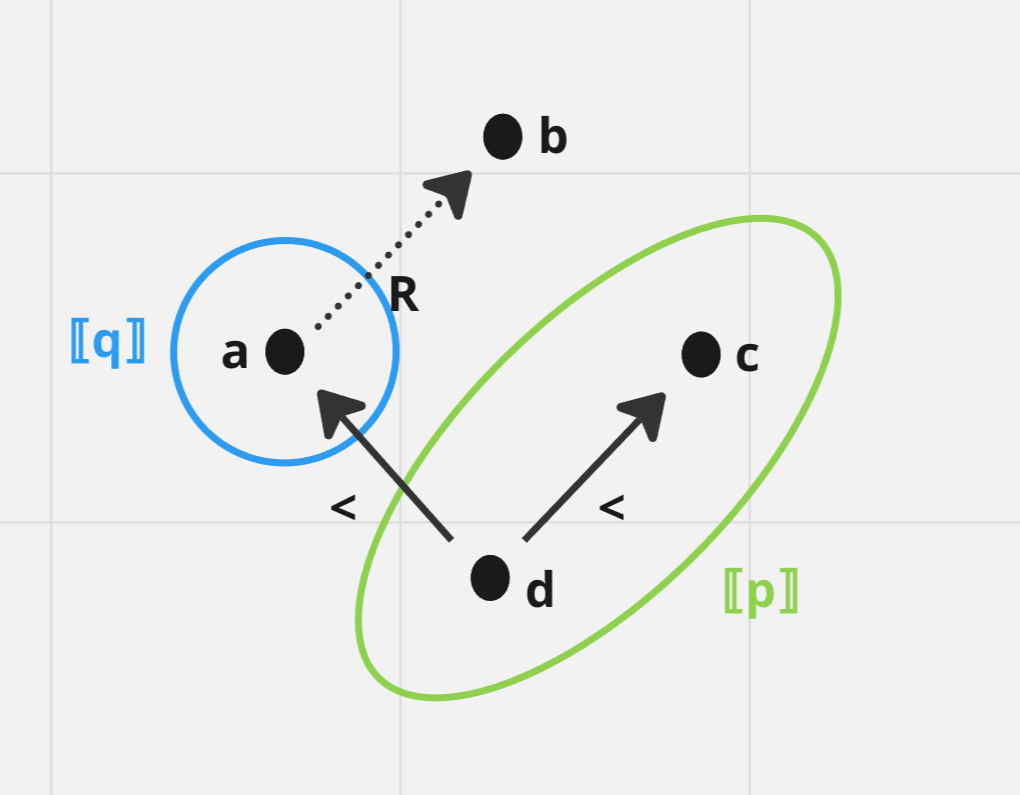
\includegraphics[scale=0.2]{4-22-24-mockup.png}
    \end{center}

    Since $\Update{p} q \leftrightarrow q$ is valid, $\semantics{q}_{\Model^\star_p} = \semantics{q}_\Model = \set{a}$.  We pick $w$ to be $a$: $a$ is $\leq$-minimal over $\semantics{q}_{\Model^\star_p}$, and so $\Model, a \Vdash \Update{p} \Typ{q}$.
    
    However, $\Model, a \not \Vdash \Typ{(q \land (\Typ{p} \lor \Know{(\Typ{p} \lor \Typ{q})}))}$.  If it did, then by reflexivity of $\Typ$ we would have $\Model, a \Vdash q \land (\Typ{p} \lor \Know{(\Typ{p} \lor \Typ{q})})$.  But $a$ does not satisfy the right conjunct.  First, $\Model, a \not \Vdash \Typ{p}$ (since $a$ is not a $\leq$-minimal element of $\semantics{p}$).  And second, there \emph{is} $b$ with $a{R}b$ such that $b$ is not a $\leq$-minimal element of either $\semantics{p}$ \emph{or} $\semantics{q}$.  So $\Model, b \not \Vdash \Typ{p} \lor \Typ{q}$, and thus $\Model, a \not \Vdash \Know{(\Typ{p} \lor \Typ{q})}$. \qedhere
\end{proof}

\paragraph*{Discussion.} This immediately rules out lexicographic upgrade, conservative upgrade, and other variants, since these update policies just re-order the plausibility relation $\leq$.  The proof also shows that $\Update{P} \varphi \leftrightarrow \varphi$ rules out any upgrade that just re-assigns propositions (i.e.\ modifies $V$).  We might instead consider updates that add or remove states or change the knowledge relation $R$, but we have to be very careful --- for example, conditionalization (i.e.\ public announcement $[!P]$ for a single agent) is also ruled out by $\Update{P} \varphi \leftrightarrow \varphi$ as well as $\Update{P} \Know{\varphi} \leftrightarrow \Know{\Update{P} \varphi}$.

I've considered looking at neighborhood models (e.g.\ evidence models) to model this update.  It's not clear to me what the neighborhood semantics for $\TypNoArgs$ should be, and I'm currently trying to find out.  What are your thoughts?

\printbibliography
\end{document}
